% vim: set textwidth=120:

% Example CV based on the 1.5-column-cv template. Main features:
% * uses the Roboto font family and IcoMoon icon set;
% * doesn't use colours, different font weights are used instead for styling;
% * because the CV fits on one page, header and footer is empty, since there isn't much useful info to put there;
% * includes a photo.
\documentclass[a4paper,10pt]{article}


% package imports
% ---------------

\usepackage[british]{babel} % for correct language and hyphenation and stuff
\usepackage{calc}           % for easier length calculations (infix notation)
\usepackage{enumitem}       % for configuring list environments
\usepackage{fancyhdr}       % for setting header and footer
\usepackage{fontspec}       % for fonts
\usepackage{geometry}       % for setting margins (\newgeometry)
\usepackage{graphicx}       % for pictures
\usepackage{microtype}      % for microtypography stuff
\usepackage{xcolor}         % for colours
\usepackage{hyperref}
\hypersetup{
    colorlinks=true,
    linkcolor=blue,
    filecolor=magenta,      
    urlcolor=blue,
}

% margin and column widths
% ------------------------

% margins
\newgeometry{left=15mm,right=15mm,top=13.5mm,bottom=13.5mm}

% width of the gap between left and right column
\newlength{\cvcolumngapwidth}
\setlength{\cvcolumngapwidth}{3.5mm}

% left column width
\newlength{\cvleftcolumnwidth}
\setlength{\cvleftcolumnwidth}{44.5mm}

% right column width
\newlength{\cvrightcolumnwidth}
\setlength{\cvrightcolumnwidth}{\textwidth-\cvleftcolumnwidth-\cvcolumngapwidth}

% set paragraph indentation to 0, because it screws up the whole layout otherwise
\setlength{\parindent}{0mm}


% style definitions
% -----------------
% style categories explanation:
% * \cvnameXXX is used for the name;
% * \cvsectionXXX is used for section names (left column, accompanied by a horizontal rule);
% * \cvtitleXXX is used for job/education titles (right column);
% * \cvdurationXXX is used for job/education durations (left column);
% * \cvheadingXXX is used for headings (left column);
% * \cvmainXXX (and \setmainfont) is used for main text;
% * \cvruleXXX is used for the horizontal rules denoting sections.

% font families
\defaultfontfeatures{Ligatures=TeX} % reportedly a good idea, see https://tex.stackexchange.com/a/37251

\newfontfamily{\cvnamefont}{Roboto Medium}
\newfontfamily{\cvsectionfont}{Roboto Medium}
\newfontfamily{\cvtitlefont}{Roboto Regular}
\newfontfamily{\cvdurationfont}{Roboto Light Italic}
\newfontfamily{\cvheadingfont}{Roboto Regular}
\setmainfont{Roboto Light}

% colours
\definecolor{cvnamecolor}{HTML}{000000}
\definecolor{cvsectioncolor}{HTML}{000000}
\definecolor{cvtitlecolor}{HTML}{000000}
\definecolor{cvdurationcolor}{HTML}{000000}
\definecolor{cvheadingcolor}{HTML}{000000}
\definecolor{cvmaincolor}{HTML}{000000}
\definecolor{cvrulecolor}{HTML}{000000}

\color{cvmaincolor}

% styles
\newcommand{\cvnamestyle}[1]{{\Large\cvnamefont\textcolor{cvnamecolor}{#1}}}
\newcommand{\cvsectionstyle}[1]{{\normalsize\cvsectionfont\textcolor{cvsectioncolor}{#1}}}
\newcommand{\cvtitlestyle}[1]{{\large\cvtitlefont\textcolor{cvtitlecolor}{#1}}}
\newcommand{\cvdurationstyle}[1]{{\small\cvdurationfont\textcolor{cvdurationcolor}{#1}}}
\newcommand{\cvheadingstyle}[1]{{\normalsize\cvheadingfont\textcolor{cvheadingcolor}{#1}}}


% inter-item spacing
% ------------------

% vertical space after personal info and standard CV items
\newlength{\cvafteritemskipamount}
\setlength{\cvafteritemskipamount}{4mm plus 1.25mm minus 1.25mm}

% vertical space after sections
\newlength{\cvaftersectionskipamount}
\setlength{\cvaftersectionskipamount}{1.5mm plus 0.5mm minus 0.5mm}

% extra vertical space to be used when a section starts with an item with a heading (e.g. in the skills section),
% so that the heading does not follow the section name too closely
\newlength{\cvbetweensectionandheadingextraskipamount}
\setlength{\cvbetweensectionandheadingextraskipamount}{0.75mm plus 0.25mm minus 0.25mm}


% intra-item spacing
% ------------------

% vertical space after name
\newlength{\cvafternameskipamount}
\setlength{\cvafternameskipamount}{2.5mm plus 0.75mm minus 0.75mm}

% vertical space after personal info lines
\newlength{\cvafterpersonalinfolineskipamount}
\setlength{\cvafterpersonalinfolineskipamount}{1.75mm plus 0.5mm minus 0.5mm}

% vertical space after titles
\newlength{\cvaftertitleskipamount}
\setlength{\cvaftertitleskipamount}{0.75mm plus 0.25mm minus 0.25mm}

% value to be used as parskip in right column of CV items and itemsep in lists (same for both, for consistency)
\newlength{\cvparskip}
\setlength{\cvparskip}{0.5mm plus 0.125mm minus 0.125mm}

% set global list configuration (use parskip as itemsep, and no separation otherwise)
\setlist{parsep=0mm,topsep=0mm,partopsep=0mm,itemsep=\cvparskip}


% CV commands
% -----------

% creates a "personal info" CV item with the given left and right column contents, with appropriate vertical space after
% @param #1 left column content (should be the CV photo)
% @param #2 right column content (should be the name and personal info)
\newcommand{\cvpersonalinfo}[2]{
    % left and right column
    \begin{minipage}[t]{\cvleftcolumnwidth}
        \vspace{0mm} % XXX hack to align to top, see https://tex.stackexchange.com/a/11632
        \raggedleft #1
    \end{minipage}% XXX necessary comment to avoid unwanted space
    \hspace{\cvcolumngapwidth}% XXX necessary comment to avoid unwanted space
    \begin{minipage}[t]{\cvrightcolumnwidth}
        \vspace{0mm} % XXX hack to align to top, see https://tex.stackexchange.com/a/11632
        #2
    \end{minipage}

    % space after
    \vspace{\cvafteritemskipamount}
}

% typesets a name, with appropriate vertical space after
% @param #1 name text
\newcommand{\cvname}[1]{
    % name
    \cvnamestyle{#1}

    % space after
    \vspace{\cvafternameskipamount}
}

% typesets a line of personal info beginning with an icon, with appropriate vertical space after
% @param #1 parameters for the \includegraphics command used to include the icon
% @param #2 icon filename
% @param #3 line text
\newcommand{\cvpersonalinfolinewithicon}[3]{
    % icon, vertically aligned with text (see https://tex.stackexchange.com/a/129463)
    \raisebox{.5\fontcharht\font`E-.5\height}{\includegraphics[#1]{#2}}
    % text
    #3

    % space after
    \vspace{\cvafterpersonalinfolineskipamount}
}

% creates a "section" CV item with the given left column content, a horizontal rule in the right column, and with
% appropriate vertical space after
% @param #1 left column content (should be the section name)
\newcommand{\cvsection}[1]{
    % left and right column
    \begin{minipage}[t]{\cvleftcolumnwidth}
        \raggedleft\cvsectionstyle{#1}
    \end{minipage}% XXX necessary comment to avoid unwanted space
    \hspace{\cvcolumngapwidth}% XXX necessary comment to avoid unwanted space
    \begin{minipage}[t]{\cvrightcolumnwidth}
        \textcolor{cvrulecolor}{\rule{\cvrightcolumnwidth}{0.3mm}}
    \end{minipage}

    % space after
    \vspace{\cvaftersectionskipamount}
}

% creates a standard, multi-purpose CV item with the given left and right column contents, parskip set to cvparskip
% in the right column, and with appropriate vertical space after
% @param #1 left column content
% @param #2 right column content
\newcommand{\cvitem}[2]{
    % left and right column
    \begin{minipage}[t]{\cvleftcolumnwidth}
        \raggedleft #1
    \end{minipage}% XXX necessary comment to avoid unwanted space
    \hspace{\cvcolumngapwidth}% XXX necessary comment to avoid unwanted space
    \begin{minipage}[t]{\cvrightcolumnwidth}
        \setlength{\parskip}{\cvparskip} #2
    \end{minipage}

    % space after
    \vspace{\cvafteritemskipamount}
}

% typesets a title, with appropriate vertical space after
% @param #1 title text
\newcommand{\cvtitle}[1]{
    % title
    \cvtitlestyle{#1}

    % space after
    \vspace{\cvaftertitleskipamount}
    % XXX need to subtract cvparskip here, because it is automatically inserted after the title "paragraph"
    \vspace{-\cvparskip}
}


% header and footer
% -----------------

% set empty header and footer
\pagestyle{empty}



% preamble end/document start
% ===========================

\begin{document}


% personal info
% -------------

\cvpersonalinfo{
    % photo
    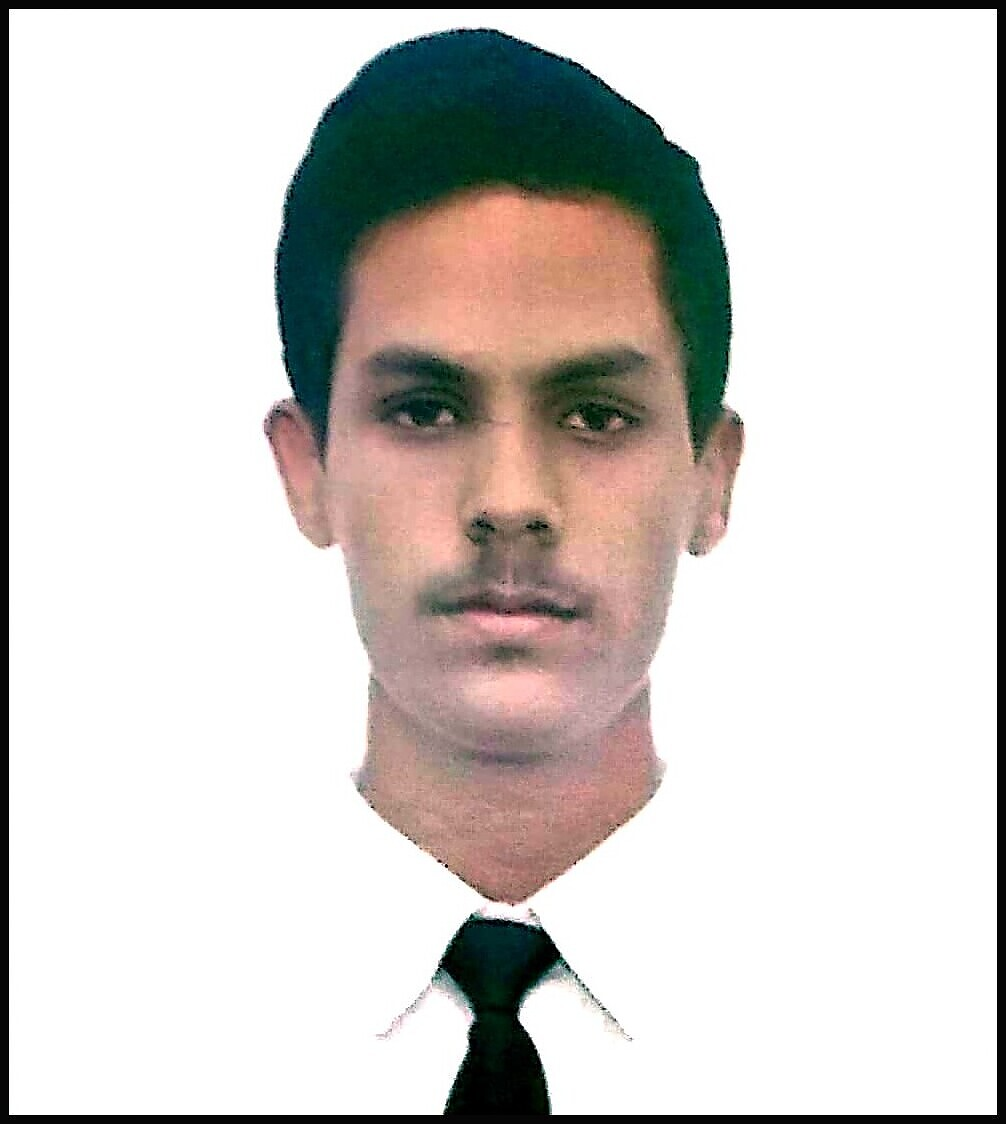
\includegraphics[height=36mm]{new2.jpg}
}{
    % name
    \cvname{Devansh Singh Rathore}

    % address
    \cvpersonalinfolinewithicon{height=4mm}{072-location.pdf}{
        House No. C-1013, Indira Nagar, Near Church, Lucknow-226016
    }

    % phone number
    \cvpersonalinfolinewithicon{height=4mm}{067-phone.pdf}{
        +91 81990\,63566\
    }

    % email address
    \cvpersonalinfolinewithicon{height=4mm}{070-envelop.pdf}{
        \href{mailto:rathoredevansh08@gmail.com}{rathoredevansh08@gmail.com}
    }

    % LinkedIn account
    \cvpersonalinfolinewithicon{height=4mm}{458-linkedin.pdf}{
        \url{https://www.linkedin.com/in/devansh-singh-rathore-b378b914b/}
    }
    
    % Github account
    \cvpersonalinfolinewithicon{height=4mm}{github.png.pdf}{
        \url{https://github.com/RathoreDevansh08}
    }

    % date of birth
    Date of Birth:  19 June 1999
}


% work experience
% ---------------

%\cvsection{WORK EXPERIENCE}

% Fake Company 2
%\cvitem{
%    \cvdurationstyle{January 2019 -- present}
%}{
%    \cvtitle{Graduate Engineer Trainee}
%
%    NEC Technologies Pvt. Ltd., Sector 135, Noida, Uttar Pradesh

%    \begin{itemize}[leftmargin=*]
%        \item Working on Openshift, Kubernetes, GoLang and %Openstack.
%    \end{itemize}
%}


% education
% ---------

\cvsection{EDUCATION}

% master's
\cvitem{
    \cvdurationstyle{2017 -- Present}
}{
    \cvtitle{B.Tech. - Computer Science and Engineering}

    From Indian Institute of Technology, Palakkad, Kerala

    \begin{itemize}[leftmargin=*]
        \item CGPA: 8.31 (Current)
        \item Elective Courses: Cryptography | Functional Programming | Digital Image Processing | Abstract Algebra | Numerical Analysis 
    \end{itemize}
}

% bachelor's
\cvitem{
    \cvdurationstyle{2016 -- 2017}
}{
    \cvtitle{Class XII}

    From O.P. Jindal Modern School, Hisar, Haryana

    \begin{itemize}[leftmargin=*]
        \item Board: Central Board of Secondary Education (CBSE)
        \item Percentage: 91.4\%
    \end{itemize}
}

% bachelor's
\cvitem{
    \cvdurationstyle{2014 -- 2015}
}{
    \cvtitle{Class X}

    From Delhi Public School, Aligarh, Uttar Pradesh

    \begin{itemize}[leftmargin=*]
        \item Board: Central Board of Secondary Education (CBSE)
        \item CGPA: 10
    \end{itemize}
}


\cvsection{EXPERIENCE}

\vspace{\cvbetweensectionandheadingextraskipamount}

\cvitem{
    \cvdurationstyle{June 2020 -- Aug 2020}
}{
    \cvtitle{GE Healthcare - Software Intern}

    \begin{itemize}[leftmargin=*]
        \item Exploration of PyCharm Plugin Development on IntelliJ IDEA, using Gradle, Java.
        \item Development of Federated Learning server-client paradigm using Tensorflow, RESTful-service (REST API), Python Flask, MySQL.
    \end{itemize}
}

% skills
% ------

\cvsection{TECHNICAL SKILLS}

\vspace{\cvbetweensectionandheadingextraskipamount}

\cvitem{
    \cvheadingstyle{Programming Languages}
}{
    
    C++, C, Python, Javascript, Haskell, Standard ML (Functional Programming)

}
\cvitem{
    \cvheadingstyle{Competitive Programming}
}{
    
   \href{https://codeforces.com/profile/DSR}{Codeforces}, \href{https://www.codechef.com/users/devansh08}{CodeChef}, \href{https://uhunt.onlinejudge.org/id/1019683}{UVa}, \href{https://www.hackerrank.com/rathoredevansh}{Hackerrank}
}

\cvitem{
    \cvheadingstyle{Deep Learning}
}{
    Completed Deep Learning online specialisation course, offered by Stanford University at coursera.org
}

\cvitem{
    \cvheadingstyle{Machine Learning}
}{
    Completed Machine Learning online course, offered by Stanford University at coursera.org
}

\cvitem{
    \cvheadingstyle{Web Development and Database}
}{
   Python Flask, REST API, CSS, HTML, MySQL
}

\cvitem{
    \cvheadingstyle{Image Processing and OpenCV}
}{
    
    Source: Digital Image Processing course (EE5005), OpenCV documentaries online, Data Analysis Club 
    
}

\cvitem{
    \cvheadingstyle{Basic Android Tracks}
}{
    
   Completed Basic Android Tracks online course offered in Google India Scholarship program 2018 at udacity.com
}

\cvsection{PROJECTS}

\vspace{\cvbetweensectionandheadingextraskipamount}

\cvitem{
    \cvdurationstyle{Jan 2020 -- July 2020}
}{
    \cvtitle{Language Server for Standard ML language}

    \begin{itemize}[leftmargin=*]
        \item Built a Language Server for Standard ML, with editing features like autocomplete, hover for IDEs.

        \item \href{https://bitbucket.org/Shruti_Umat/language-server-for-sml/src/master/}{Bitbucket Repository Link}
    \end{itemize}
}


\cvitem{
    \cvdurationstyle{May 2019 -- Nov 2019}
}{
    \cvtitle{Petrichor-2020 Fest website and CA portal development  }

    \begin{itemize}[leftmargin=*]
        \item Developed front end of Petrichor-2020 (Annual Techno-Cultural fest of IIT Palakkad) website and its CA- Portal.
        \item \href{http://petrichor-ca.herokuapp.com/}{Website Link}
    \end{itemize}
}

\cvitem{
    \cvdurationstyle{Oct 2018 -- Nov 2018}
}{
    \cvtitle{Garbage Management Mini Project using Verilog}
    \begin{itemize}[leftmargin=*]
        \item Simulation of an efficient garbage collection system (using Dijkstra's shortest path algorithm) - Verilog
        \item \href{https://github.com/RathoreDevansh08/Garbage\_Management\_MiniProject}{Github Repository Link} 
        
    \end{itemize}
}

\cvitem{
    \cvdurationstyle{July 2018 -- August 2018}
}{
    \cvtitle{Face Recognition Project}

    \begin{itemize}[leftmargin=*]
        \item Developed a Face recognition Python program for automated attendance system that recognizes and predicts the person in image. Built using Deep Learning methods (CNN, Triplet Loss algorithm).
        \item \href{https://github.com/RathoreDevansh08/CSpuare\_FaceRecognition}{Github Repository Link}
        
    \end{itemize}
}

\cvitem{
    \cvdurationstyle{Jan 2018 -- Feb 2018}
}{
    \cvtitle{Cartoonifier using OpenCV}
    \begin{itemize}[leftmargin=*]
        \item Developed a program to cartoonify an image using image processing and OpenCV (Bilateral filter, Laplacian filter, Sobel Edge Detection).
        \item \href{https://github.com/RathoreDevansh08/Cartoonifier}{Github Repository Link}
        
    \end{itemize}
}

\cvitem{
    \cvdurationstyle{Dec 2017 -- Mar 2018}
}{
    \cvtitle{Online E - Challan system}
    \begin{itemize}[leftmargin=*]
        \item Developed an automated online e - challan web application with additional ML applications, for Smart India Hackathon 2018.
        \item \href{http://iit.pscquestion.in/}{Website Link}
        
    \end{itemize}
}



\cvsection{TRAINING AND WORKSHOPS}

\vspace{\cvbetweensectionandheadingextraskipamount}

\cvitem{
    \cvdurationstyle{Nov 2018 -- Dec 2018}
}{

    \cvtitle{ Inter IIT Tech meet 2018 (Star Cluster Identifier, PlutoX Hackathon) at IIT Bombay}
}

\cvitem{
    \cvdurationstyle{Jun 2018 -- July 2018}
}{
    \cvtitle{Deep Learning at Stanford University (online)}
}

\cvitem{
    \cvdurationstyle{Jun 2018}
}{
    \cvtitle{MyCaptain Artificial Intelligence (The CLIMBER program) at MyCaptain (online)}
}

\cvitem{
    \cvdurationstyle{Jan 2018}
}{
    \cvtitle{Kaizen Internet Of Things Workshop by LemaLabs}
}

\cvitem{
    \cvdurationstyle{Dec 2017 -- Feb 2018}
}{
    \cvtitle{Machine Learning at Stanford University (online)}
}


% education
% ---------

\cvsection{ACHIEVEMENTS}

\vspace{\cvbetweensectionandheadingextraskipamount}

\cvitem{
    \cvheadingstyle{}
}{
    
    \begin{itemize}[leftmargin=*]
    
        \item \textbf{Google Hashcode 2020:} Team achieved 1436th place(world ranking) in Hash Code 2020 Online Qualification round
        \item \textbf{ICPC 2019-20:} Our team achieved rank 244 in online preliminary round and qualified for onsite round. Achieved rank 28 in Asia region Kanpur site, rank 251 in Asia region Amritapuri site.
        \item \textbf{Codechef Snackdown 2019:} Qualified for online contest round 1B
        \item \textbf{Smart India Hackathon 2018:} Qualified for grand final round of SIH-2018
        \item \textbf{Google India Scholarship Challenge 2018:} Selected for the program, completed Basic Android Tracks online course
        
    \end{itemize}

    
}

\cvsection{POSITION OF RESPONSIBILITIES}

\vspace{\cvbetweensectionandheadingextraskipamount}

\cvitem{
    \cvdurationstyle{Dec 2019 -- Jan 2020}
}{
    \cvtitle{Organizer of Data Analytics Contest for Petrichor-2020 Fest}
}

\cvitem{
    \cvdurationstyle{May 2019 -- Dec 2019}
}{
    \cvtitle{Member of Web Creative Team for Petrichor-2020 Fest}
}

\cvitem{
    \cvdurationstyle{Aug 2018 -- April 2019}
}{
    \cvtitle{Head of Data Analysis Club, IIT Palakkad}
}

% additional info
% ---------------

\cvsection{EXTRACURRICULAR ACTIVITIES}

\vspace{\cvbetweensectionandheadingextraskipamount}

\cvitem{
    \cvheadingstyle{}
}{
    
    \begin{itemize}[leftmargin=*]
        \item \textbf{Chess:} Active participant in institute Chess competitions
        \item \textbf{NSO (Table Tennis):} Completed 40 hours of Table Tennis training
        \item \textbf{EBSB cultural program:} Participant
        
    \end{itemize}

    
}


\end{document}